\documentclass[a4paper, 12pt, fleqn]{report}

\usepackage{graphicx}
\usepackage{geometry}
\usepackage{caption}
\geometry{a4paper, margin=1in}
\usepackage{amsmath}
\usepackage{amssymb}
\usepackage{multirow}
\usepackage{hyperref}
\usepackage{float}
\usepackage{pgfplots}
\pgfplotsset{compat=1.17}
\usepackage{nameref}

\begin{document}

% Cover page
\begin{titlepage}
    \centering
    \vspace*{1cm}
    \includegraphics[width=0.4\textwidth]{uc_logo.jpg}

    {\Huge\bfseries Artificial Inteligence Fundamentals Lab Assignment 2 - Stage 2\par}
    \vspace{0.1cm}
    {\Large\itshape The evolution of Lunar Lander \par}
    \vfill
    \vfill
        \begin{center}
            \large
            \textbf{Members: \\}
            Miguel Castela 2022212972, PL1\\
            Miguel Martins 2022213951, PL1\\
            Nuno Batista 2022216127, PL1
    \end{center}
    
    \vfill
    
    {\large March, 2025 \par}
\end{titlepage}

% Table of contents
\renewcommand{\contentsname}{Table of Contents}
\tableofcontents
\newpage

% Sections
\section*{\fontsize{16}{20}\selectfont Perceptions}
\addcontentsline{toc}{section}{Perceptions}

\begin{table}[h!]
\centering
\begin{tabular}{p{3cm} p{3cm} p{10cm}}
\textbf{Perception} & \textbf{Name} & \textbf{Description} \\[15pt]
observation[0] & $x$ & Horizontal position relative to the landing platform. ($x < 0$ if the ship is to the left of the platform and $x > 0$ otherwise)\\[10pt]
observation[1] & $y$ & Vertical position, relative to the ground. \\[10pt]
observation[2] & $v_x$ & Horizontal velocity. Negative when the ship is going to the left and positive when its going to the right\\[10pt]
observation[3] & $v_y$ & Vertical velocity. Negative when the ship is going down and positive when its going up \\[10pt]
observation[4] & $\theta$ & Ship's orientation ($\theta < 0$ if the ship is tilted to the left of the platform and $\theta > 0$ otherwise) \\[10pt]
observation[5] & $v_\theta$ & Angular velocity ($v_\theta > 0$ if the ship is rotating counter-clockwise and $v_\theta < 0$ if cloclwise)\\[10pt]
observation[6] & $RLT$ & Boolean: $True$ if the right leg is in contact with the ground, $False$ otherwise \\[10pt]
observation[7] & $LLT$ & Boolean: $True$ if the left leg is in contact with the ground, $False$ otherwise \\[10pt]
\end{tabular}
\caption{Perceptions Declaration}
\label{tab:perceptions}
\end{table} 



\section*{\fontsize{16}{20}\selectfont Action Declaration}
\addcontentsline{toc}{section}{Actions}


\begin{table}[h!]
\centering
\begin{tabular}{|p{1cm}|p{4cm}|p{11cm}|}
\hline
\multicolumn{1}{|c|}{\textbf{Name}} & \multicolumn{1}{c|}{\textbf{Action}} & \multicolumn{1}{c|}{\textbf{Description}} \\ \hline
Mm & Controls the main motor. & Activated for values larger than 0.5, linearly increases the acceleration until reaching the maximum value of 1. \\ \hline
Lm & Controls the left motor. & Activated for values larger than 0.5, the left motor is activated, rotating the ship to the right. It's acceleration linearly increases until reaching the maximum value of 1.\\ \hline
Rm & Controls the right motor. & Activated for values lower than -0.5, the right motor is activated, rotating the ship to the left. It's acceleration linearly increases until reaching the maximum value of -1. \\ \hline
\end{tabular}
\caption{Actions declaration}
\label{tab:actions}
\end{table}

\newpage
\section*{\fontsize{16}{20}\selectfont Windless Environment}
\addcontentsline{toc}{section}{Windless Environment}

In the first stage of our evolutionary algorithm, we focused on implementing four key components: parent selection, crossover, 
mutation, and the objective function. Below is a detailed explanation of each mechanism.


\subsection*{Parent Selection}
\addcontentsline{toc}{subsection}{Parent Selection}

We implemented a selection of strategies to select parents from the population:

\begin{itemize}
    \item \textbf{Roulette Selection}: Roulette selection is a method used to select individuals from the population based on their fitness values. The probability of selecting an individual is proportional to its fitness. Individuals with higher fitness values have a higher chance of being selected.

\noindent
To implement this, we first calculate the total fitness of the population. Then, each individual's selection probability is determined by dividing its fitness by the total. A random number is then generated, and one individual is selected based on these probabilities, simulating a spin of a roulette wheel where larger fitness values occupy more space on the wheel.

\noindent
This method encourages the selection of fitter individuals while still allowing those with lower fitness a non-zero chance of being selected, which helps preserve diversity in the population. If all individuals have zero fitness, selection defaults to uniform random selection to prevent errors.
    \item \textbf{Tournament of 2}: This method involves randomly selecting two individuals from the population to form a tournament. These individuals are compared based on their fitness values, and the one with the higher fitness is selected as the parent. As this approach always picks the best of the two without any added randomness, it is a purely exploitative strategy.

\noindent
While it is simple and computationally efficient, the lack of stochasticity can lead to quicker convergence but also increases the risk of getting trapped in local optima due to reduced diversity in selection.

    \item \textbf{Tournament of 5}: We randomly select five individuals from the population to form a tournament. These individuals are then sorted based on their fitness values in descending order (so that the best-performing individual appears first). To introduce controlled randomness and maintain genetic diversity, we use a probabilistic selection mechanism:

    \begin{itemize}
        \item The best individual is selected with a probability of \(P\).
        \item The second-best is selected with a probability of \(P \times (1 - P)\).
        \item The third-best is selected with a probability of \(P \times (1 - P)^2\).
        \item If none of these probabilities match, a random individual from the tournament is selected.
    \end{itemize}
\noindent
For the simulations conducted, we set the probability \(P\) to 0.9.
This method balances exploitation (favoring the best individuals) with exploration (occasionally selecting weaker individuals) to avoid premature convergence.
\end{itemize}

\subsection*{Crossover}
\addcontentsline{toc}{subsection}{Crossover}
We used a single-point crossover method, where a random index is selected along the genotype—representing the individual's weights. 
The offspring's genotype is formed by taking the first segment of one parent's genotype (up to the crossover point) and combining it with the remaining segment from the other parent (starting from the crossover point). 
This technique enables the offspring to inherit characteristics from both parents, encouraging genetic diversity in the following generation.
We tested two crossover probabilities: 0.5 and 0.9.

\subsection*{Mutation}
\addcontentsline{toc}{subsection}{Mutation}

We implemented Gaussian mutation to introduce small random variations in the genotype of an individual, preventing the algorithm from converging prematurely. 
For each gene in the genotype, there is a probability ($PROB\_MUTATION$) that the gene will be modified. 
If selected for mutation, a random value drawn from a Gaussian distribution centered at 0 with a given standard deviation ($STD\_DEV$) is added to the gene. 
To ensure that gene values remain within acceptable limits, the mutated value is clamped to stay within the range [-1, 1]. 
This mutation mechanism helps maintain genetic variation and allows the algorithm to explore new areas of the search space.
We tested two mutation probabilities: 0.008 and 0.05.

\newpage
\subsection*{Evolution of the objective function and score progression}
\addcontentsline{toc}{subsection}{Evolution of the objective function and score progression}
\noindent
The objective function is designed to evaluate the performance of the lunar lander in terms of its landing accuracy and safety.\\
Firstly, we added a \textbf{penalty for the ship's vertical velocity}:

{\scriptsize
\begin{equation}
    \centering
    \text{return} \left( 
        - |x| 
        - |y| 
        - |v_y|, 
        \text{check\_successful\_landing}(\text{observation})
    \right)
\end{equation}
}


\noindent
Independent of the Mutation, Crossover rate and Tournament type used, this resulted in a 0.0 hitrate and a mild negative fitness ($\approx -0.03$), so we added a \textbf{reward when the ship has both legs touching the ground} ($both\_legs\_touching$). This was not enough to drive up the hitrate (it only caused a 2\% increase), so we also added an \textbf{angular velocity penalty}:

{\scriptsize
\begin{equation}
    \centering
    \begin{array}{l}
        \text{legs\_touching} = (\text{contact\_left} = 1 \land \text{contact\_right} = 1) \\[0.5em]
        \text{return} \left( 
            - |x| 
            - |y| 
            + (\text{legs\_touching}) 
            - |v_y| 
            - |v_\theta|, 
            \text{check\_successful\_landing}(\text{observation})
        \right)
    \end{array}
\end{equation}
}


\noindent
This change resulted, in the best scenario (Prob\_Crossover = 0.9, Prob\_Mutation = 0.05 and a Tournament of 5) in a 30\% hitrate, wich showed us that the ship was able to learn to land, but not in a consistent way.\\
We then reassessed our approach and tried adding penalties and rewards inspired by our production system implementation, rewarding the more "specific" productions with higher rewards, and the more "general" productions with lower rewards. This resulted in a final generation with a fitness of about 101. 

{\scriptsize
\begin{center}
\begin{gather}
    \begin{aligned}
    & \text{stable\_orientation} = |\theta| < 0.15, \quad
      \text{on\_landing\_pad} = |x| \leq 0.2, \\
    & \text{stable\_velocity} = v_y > -0.2, \quad
     \text{stable} = \text{stable\_velocity} \land \text{stable\_orientation}, \\
    & \text{legs\_touching} = (\text{contact\_left} = 1 \land \text{contact\_right} = 1), \\
    & \text{one\_leg\_touching} = (\text{contact\_left} = 1 \lor \text{contact\_right} = 1), \\
    & \text{good\_height} = (y < 2.1), \quad
        \text{stable\_orientation\_int} =(|\theta| < 0.15), \\
    & \text{stable\_vertical\_velocity} = (|v_y| < 0.3), \quad
        \text{stable\_angular\_velocity} = (|v_\theta| < 0.3), \\
    & \text{stable\_horizontal\_velocity} = (|v_x| < 0.2), \quad
        \text{stable\_x} =(|x| < 0.2), \\
    & \text{perfect\_x} = (|x| = 0), \quad
        \text{too\_far\_x} = (|x| > 0.1), 
    \end{aligned}
\end{gather}



\begin{gather}
    \begin{aligned}
    & \text{return} \Big( 
        -|x| \cdot 100 + \text{legs\_touching} \cdot 100 + \text{one\_leg\_touching} \cdot 50 \\
    & \quad + \text{good\_height} \cdot 10 + \text{stable\_velocity} \cdot 100 + \text{stable\_orientation} \cdot 10 \\
    & \quad + \text{stable} \cdot 100 + \text{on\_landing\_pad} \cdot 100 + \text{stable\_orientation\_int} \cdot 10 \\
    & \quad + \text{stable\_vertical\_velocity} \cdot 10 + \text{stable\_angular\_velocity} \cdot 50 \\
    & \quad + \text{stable\_horizontal\_velocity} \cdot 10 + \text{stable\_x} \cdot 10 \\
    & \quad + \text{perfect\_x} \cdot 100 - \text{too\_far\_x} \cdot 100, \\
    & \quad \text{check\_successful\_landing}(\text{observation}) \Big)
    \end{aligned}
\end{gather}
\end{center}
}

    
    \noindent
    This resulted in an average of 0.01\% hitrate (occasionally it was a little higher), so we started working on branching and binary conditions.

    So, we started to define \textbf{3 different branches}, one to make the ship stable (it had to have a stable orientation and stable velocity, based on the thresholds of the prevoius function), then one to make it land on the landing pad, and one to make it land safely.
    Landig safely was a challenge, because we started noticing the ship would often hover the ground without actually landing,
    so we added a \textbf{penalty for when the ship is slowly hovering in the range of the two flags, but its legs are not touching the ground}. These changes resulted in a final fitness of about 1449.\\

{\scriptsize
\begin{center}
    \begin{align*}
    \text{legs\_touching} &= (c_L = 1 \land c_R = 1) \\
    \text{hover\_penalty} &= 
    \begin{cases} 
    -100, & \text{if } |x| < 0.2 \land |v_x| < 0.2 \land \neg (\text{legs\_touching}) \\ 
    0, & \text{otherwise} 
    \end{cases}
    \end{align*}
\end{center}
}
    
    \noindent
    We decided to maintain the penalties for the absolute values of the ship's position.
    We also maintaned the $legs\_touching$, $stable\_orientation$, $stable\_with\_less\_inpact$, $on\_landing\_pad$ and $stable\_velocity$ \textbf{rewards mentioned above}.
    \\

    \noindent
    \\
    To help make the punishment of the ship more precise, we implemented a new set of penalties based on the ship's position, velocity, and orientation. These penalties are designed to discourage dangerous behaviors during descent while rewarding controlled and precise landings.
    These include penalties for excessive angular velocity, high vertical velocity when close to the ground, and poor horizontal positioning. The penalties are applied conditionally based on the ship's state, allowing for more nuanced control over its behavior:
    \\
{\scriptsize
\begin{center}
    \begin{align*}
        & \text{very\_near\_ground} = y < 0.2 \\
        & \text{height\_factor} = 1 + \frac{2}{\max(0.1, y)} \\[0.5em]
        & \text{near\_ground} = y < 0.5 \\
        & \text{centered\_position} = |x| < 0.2 \\
        & \text{stable\_orientation} = |\theta| < 0.15
    \end{align*}
    
    \begin{align*}
        \text{penalties} = {} 
        & -800 \cdot (|\theta| > 0.6) \\
        & -500 \cdot (|v_\theta| > 1.0) \\
        & -1000 \cdot (v_y < -1.0 \land y < 1.0) \\
        & -800 \cdot (|x| > 0.8) \cdot \text{height\_factor} \\
        & -400 \cdot (|v_x| > 0.8)
    \end{align*}
    
    \begin{align*}
        & \text{if very\_near\_ground} \land \text{centered\_position} \land \text{stable\_orientation} \land |v_y| < 0.05: \\
        & \quad \text{penalties} \mathrel{-}= 300
    \end{align*}
\end{center}
}

\noindent
    While trying different ways of doing these branches and  with this hovering decision made, paired with testing with different sets of parameters made the hitrate hover about ~8.5\% with ocasional inconsistent bumps to about 80\%. A little better, but the ship was't landing consistently.
    \noindent
    \\
    \\This made us decide to \textbf{keep the stabilty branch and make the positioning branch much stronger, while enhancing the descent rate branch with high priority before the landing component}.
    This new branch reward a slower descent, this is done by checking if the descent was a safe\_descent ($vy > -0.5$), rewarding it, a very\_safe\_descent ($vy > -0.2$), rewarding it even more, and punishing the ship if it had a high vertical velocity. This resulted in a very slight increase of the hitrate.
    
    {\scriptsize
    \begin{center}
    \begin{align*}
    & \text{stable\_orientation} = |\theta| < 0.15 \\
    & \text{stable\_angular\_velocity} = |v_\theta| < 0.3 \\
    & \text{stable\_horizontal\_velocity} = |v_x| < 0.2 \\
    & \text{centered\_position} = |x| < 0.2 \\
    & \text{stability\_score} =
    500 \cdot \text{stable\_orientation} +
    300 \cdot \text{stable\_angular\_velocity} +
    200 \cdot \text{stable\_horizontal\_velocity} \\
    & \text{positioning\_score} =
    \Big( 400 \cdot \text{centered\_position} +
          300 \cdot (1 - \min(1, \tfrac{|x|}{0.5})) +
          200 \cdot (1 - \min(1, \tfrac{|v_x + 0.5x|}{0.5})) \Big)
    \cdot \text{height\_factor} \\
    \end{align*}
    \end{center}
    }

    
    \noindent
    Given the inconsistent and stochastic nature of the problem, we started to evaluate the fitness of each individual based on the average performance over 5 test runs . This helps test the ability for the agent to generalize. This approach also prevents genotypes that perform well on just one specific terrain to be passed into new generations and being cloned in future generations (given that this can misguide the evolutionary process and lead to less general, overfitted solutions). These results were avaluated in the section "Adding consistency to the fitness function".
{\scriptsize
\begin{center}
    \begin{align*}
        & \text{total\_fitness} = 0 \\
        & \text{success\_count} = 0 \\
        & \text{num\_trials} = \text{NUM\_EVALS} \\
        & \text{for } i = 1 \text{ to } \text{num\_trials}: \\
        & \quad (\text{score}, \text{success}) = \text{simulate}(\text{ind.genotype}, \text{seed} = \text{None}, \text{env}) \\
        & \quad \text{total\_fitness} \mathrel{+}= \text{score} \\
        & \quad \text{success\_count} \mathrel{+}= \text{int(success)} \\[0.5em]
        & \text{ind.fitness} = \dfrac{\text{total\_fitness}}{\text{num\_trials}} \\
        & \text{ind.success\_rate} = \dfrac{\text{success\_count}}{\text{num\_trials}}
    \end{align*}
\end{center}
}


\noindent
We kept the parameters stated above (Prob\_Crossover = 0.9, Prob\_Mutation = 0.05 and a Tournament of 5) given that these were the best performing when doing the benchmarks (as you can see in the table below)
, after adjusting the thresholds, \textbf{increasing penalties for excessive velocity, poor positioning, and unstable hovering, while rewarding behaviors that contributed to a stable descent,} we achieved a hit rate of 78.1\%.
The biggest contributors to this massive change were the
\begin{itemize}
        \item \textbf{Conditional logic for near ground,} diminiscing the rewards of the landing velocity based on the height of the ship:
        {\scriptsize
        \begin{align*}
            & \text{legs\_touching} = (c_L = 1 \land c_R = 1) \\
            & \text{near\_ground} = y < 0.5 \\
            & \text{very\_near\_ground} = y < 0.2 \\
            & \text{landing\_score} =
            \begin{cases}
                500 \cdot \text{legs\_touching} +
                200 \cdot \text{one\_leg\_touching} +
                400 \cdot \text{stable\_vertical\_velocity} +
                400 \cdot \text{centered\_position} + {} \\
                \quad 800 \cdot (-0.2 < v_y < -0.05) +
                1500 \cdot \text{legs\_touching}, 
                & \text{if near\_ground and very\_near\_ground} \\
                0, & \text{otherwise}
            \end{cases}
        \end{align*}
        }
        \item \textbf{Increased rewards for slow descents, resulting in perfect landings,} boosting the reward significantly for touching down correctly and having a good descent rate during touchdown (the new $descent\_score$ also helped).
        {\scriptsize
        \begin{align*}
        & \text{height\_factor} = 1 + \frac{2}{\max(0.1, y)} \\[0.5em]
        & \text{safe\_descent\_rate} = v_y > -0.5 \\
        & \text{very\_safe\_descent} = v_y > -0.2 \\
        & \text{descent\_score} =
        \Big( 400 \cdot \text{safe\_descent\_rate} + 
                600 \cdot \text{very\_safe\_descent} +
                300 \cdot \left(1 - \min\left(1, \tfrac{|v_y|}{1.0}\right)\right) \Big)
        \\[0.2em]
        & \qquad \cdot \text{height\_factor} \\[0.5em]
        \end{align*}
        }
        \end{itemize}

    \noindent
    After defining the penalties and rewards, we added a final score function that combines all the previous components. This function evaluates the ship's performance based on its stability, positioning, descent rate, and landing success. In the final generation these changes resulted fitness of 151739. The final score is calculated as follows:
    {\scriptsize
    \begin{center}
    \begin{align*}
        & \text{total\_score} =
          \text{stability\_score} +
          \text{positioning\_score} +
          \text{descent\_score} \\
        & \quad + \text{landing\_score} \cdot
          (\text{stable\_orientation} \cdot \text{centered\_position} \cdot \text{safe\_descent\_rate}) +
          \text{penalties} \\
        & \text{return}(\text{total\_score}, \text{check\_successful\_landing(observation)})
        \end{align*}
        \end{center}
    }



        \newpage
        \subsection*{Final score and statistic tests}
        \addcontentsline{toc}{subsection}{Final score and statistic tests}

        \subsubsection*{Final objective function}
        \addcontentsline{toc}{subsubsection}{Final objective function}

        The final objective function is a combination of the previous functions, with the addition of a penalty proportional to the number of steps taken in order to favor individuals that complete the task faster. We changed the crossover probability to 0.5, kept the mutation probability at 0.008 and the tournament type at 5, as these continued to be the best performing when doing the benchmark table tests.
        The final objective function has this code added:

        {\scriptsize
        \begin{center}
        \begin{align*}
            & \text{steps\_penalty} = -0.1 \cdot (\text{STEPS} - 1) \\
            & \text{penalties} += \text{steps\_penalty} \\[0.5em]
            & \text{total\_score} =
            \text{stability\_score} +
            \text{positioning\_score} +
            \text{descent\_score} \\
            & \quad + \text{landing\_score} \cdot
            (\text{stable\_orientation} \cdot \text{centered\_position} \cdot \text{safe\_descent\_rate}) +
            \text{stopped\_reward} \\
            & \text{total\_score} += \text{penalties}
        \end{align*}
    \end{center}
        }
        
    

\begin{table}[H]
    \centering
    \begin{tabular}{|c|c|c|c|c|c|}
    \hline
    \textbf{} & \textbf{Mutação} & \textbf{Crossover} & \textbf{Elitismo} & \textbf{Tamanho da População} & \textbf{Gerações} \\
    \hline
    Experiência 1 & 0.008 & 0.5 & \multirow{4}{*}{0} & \multirow{8}{*}{100} & \multirow{8}{*}{100} \\
    \cline{1-3}
    Experiência 2 & 0.05 & 0.5 &  &  &  \\
    \cline{1-3}
    Experiência 3 & 0.008 & 0.9 &  &  &  \\
    \cline{1-3}
    Experiência 4 & 0.05 & 0.9 &  &  &  \\
    \cline{1-4}
    Experiência 5 & 0.008 & 0.5 & \multirow{4}{*}{1} &  &  \\
    \cline{1-3}
    Experiência 6 & 0.05 & 0.5 &  &  &  \\
    \cline{1-3}
    Experiência 7 & 0.008 & 0.9 &  &  &  \\
    \cline{1-3}
    Experiência 8 & 0.05 & 0.9 &  &  &  \\
    \hline
    \end{tabular}
    \caption{Configuration of the experiments for different parameters.}
    \end{table}

    \begin{table}[H]
        \centering
        \begin{tabular}{|c|c|c|c|c|c|}
        \hline
        \textbf{Experiência} & \textbf{Hitrate} & \textbf{Score Médio} \\
        \hline
                    1 & 15.4\% & 56653.992  \\
        \hline
                    2 & 92.5\% & 141230.92  \\
        \hline
                    3 & 18.3\% & 61151.43  \\
        \hline
                    4 & 96.9\% & 146582.12 \\
        \hline
                    5 & 20.5\% & 49808.66  \\
        \hline
                    6 & 97.2\% & 148110.92 \\
        \hline
                    7 & 21.0\%  & 60213.836 \\
        \hline
                    8 & 97.9\% & 148250.92 \\
        \hline
        \end{tabular}
        \caption{Results of the experiments with different parameters.}
        \label{tab:experiments}
    \end{table}



\subsubsection{Adding consistency to the fitness function}
\addcontentsline{toc}{subsection}{Adding consistency to the fitness function}

Before evaluating fitness based on the average of 5 simulations (a decision stated above), the fitness function evolved in a highly inconsistent manner, with abrupt jumps and fluctuations.
(This is illustrated in the graph, where fitness progresses erratically.)
\begin{figure}[h!]
    \centering
    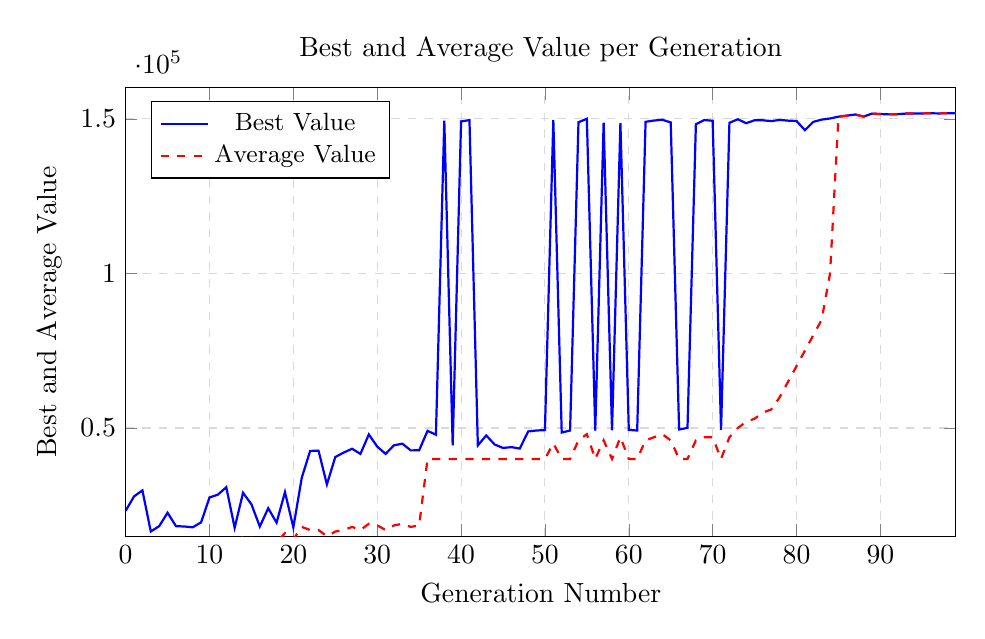
\begin{tikzpicture}
        \begin{axis}[
            width=\textwidth,
            height=0.6\textwidth,
            xlabel={Generation Number},
            ylabel={Best and Average Value},
            xmin=0, xmax=99,
            ymin=15000, ymax=160000,
            grid=major,
            grid style={dashed, gray!30},
            legend pos=north west,
            legend style={font=\small},
            title={Best and Average Value per Generation}
        ]
        % Best value in blue
        \addplot[color=blue, thick] coordinates {
            (0, 23191.59765625) (1, 27867.533203125) (2, 29810.169921875) (3, 16514.951171875)
            (4, 18247.00390625) (5, 22587.580078125) (6, 18247.783203125) (7, 18137.494140625)
            (8, 17877.458984375) (9, 19473.986328125) (10, 27533.107421875) (11, 28430.970703125)
            (12, 30852.068359375) (13, 17736.416015625) (14, 29035.548828125) (15, 25317.724609375)
            (16, 18122.939453125) (17, 24041.966796875) (18, 19385.861328125) (19, 29258.6328125)
            (20, 17825.064453125) (21, 33866.68359375) (22, 42575.47265625) (23, 42673.43359375)
            (24, 31727.150390625) (25, 40602.46484375) (26, 42046.3828125) (27, 43280.11328125)
            (28, 41620.5703125) (29, 47908.41796875) (30, 43984.46484375) (31, 41628.93359375)
            (32, 44403.91015625) (33, 44914.4375) (34, 42758.41015625) (35, 42774.453125)
            (36, 49069.33984375) (37, 47830.546875) (38, 149402.5) (39, 44421.1484375)
            (40, 149145.8125) (41, 149579.890625) (42, 44361.359375) (43, 47589.5078125)
            (44, 44663.2734375) (45, 43540.703125) (46, 43810.125) (47, 43336.53515625)
            (48, 48888.109375) (49, 49194.6015625) (50, 49308.27734375) 
            (51, 149559.65625) (52, 48523.15234375) (53, 49179.4921875) (54, 148886.90625)
            (55, 150008.453125) (56, 49168.5546875) (57, 148772.234375) (58, 49219.0234375)
            (59, 148594.015625) (60, 49385.140625) (61, 49179.58984375) (62, 149018.71875)
            (63, 149437.078125) (64, 149680.84375) (65, 148821.359375) (66, 49514.1875)
            (67, 50037.33984375) (68, 148228.8125) (69, 149601.328125) (70, 149361.546875)
            (71, 49398.26171875) (72, 148700.375) (73, 149854.71875) (74, 148573.6875)
            (75, 149519.546875) (76, 149511.25) (77, 149253.53125) (78, 149636.8125)
            (79, 149401.234375) (80, 149291.09375) (81, 146329.90625) (82, 148997.375)
            (83, 149746.046875) (84, 150102.859375) (85, 150675.75) (86, 151020.671875)
            (87, 151388.484375) (88, 150708.84375) (89, 151677.75) (90, 151531.265625)
            (91, 151429.0625) (92, 151485.15625) (93, 151677.65625) (94, 151679.8125)
            (95, 151741.375) (96, 151775.140625) (97, 151737.84375) (98, 151784.1875)
            (99, 151828.625)
        };

        % Average value in red dashed (replace these with your real averages)
        \addplot[color=red, thick, dashed] coordinates {
            (0, 7000) (1, 9000) (2, 11000) (3, 8000) (4, 8500) (5, 10000) (6, 9500) (7, 9000)
            (8, 9500) (9, 10500) (10, 13000) (11, 13500) (12, 14000) (13, 11000) (14, 15000)
            (15, 14500) (16, 13000) (17, 14000) (18, 13000) (19, 16000) (20, 14000) (21, 18000)
            (22, 17000) (23, 17000) (24, 15000) (25, 16500) (26, 17000) (27, 18000) (28, 17000)
            (29, 19000) (30, 18500) (31, 17000) (32, 18500) (33, 19000) (34, 18000) (35, 18500)
            (36, 40000) (37, 40000) (38, 40000) (39, 40000) (40, 40000) (41, 40000) (42, 40000)
            (43, 40000) (44, 40000) (45, 40000) (46, 40000) (47, 40000) (48, 40000) (49, 40000)
            (50, 40000) (51, 45000) (52, 40000) (53, 40000) (54, 46000) (55, 48000) (56, 40000)
            (57, 46000) (58, 40000) (59, 47000) (60, 40000) (61, 40000) (62, 46000) (63, 47000)
            (64, 48000) (65, 46000) (66, 40000) (67, 40000) (68, 46000) (69, 47000) (70, 47000)
            (71, 40000) (72, 47000) (73, 50000) (74, 52000) (75, 53000) (76, 55000) (77, 56000)
            (78, 60000) (79, 65000) (80, 70000) (81, 75000) (82, 80000) (83, 85000) (84, 100000)
            (85, 150675.75) (86, 151020.671875)
            (87, 151388.484375) (88, 150708.84375) (89, 151677.75) (90, 151531.265625)
            (91, 151429.0625) (92, 151485.15625) (93, 151677.65625) (94, 151679.8125)
            (95, 151741.375) (96, 151775.140625) (97, 151737.84375) (98, 151784.1875)
            (99, 151828.625)

        };

        \legend{Best Value, Average Value}
        \end{axis}
    \end{tikzpicture}
    \caption{Best and Average Value per Generation}
    \label{fig:best_avg_value_per_generation}
\end{figure}

\noindent
\\After introducing the averaging over 5 simulations, although the fitness curve remains somewhat wobbly due to the stochastic nature of the problem, it becomes significantly more consistent and closer to being monotonically increasing.

\begin{figure}[h!]
    \centering
    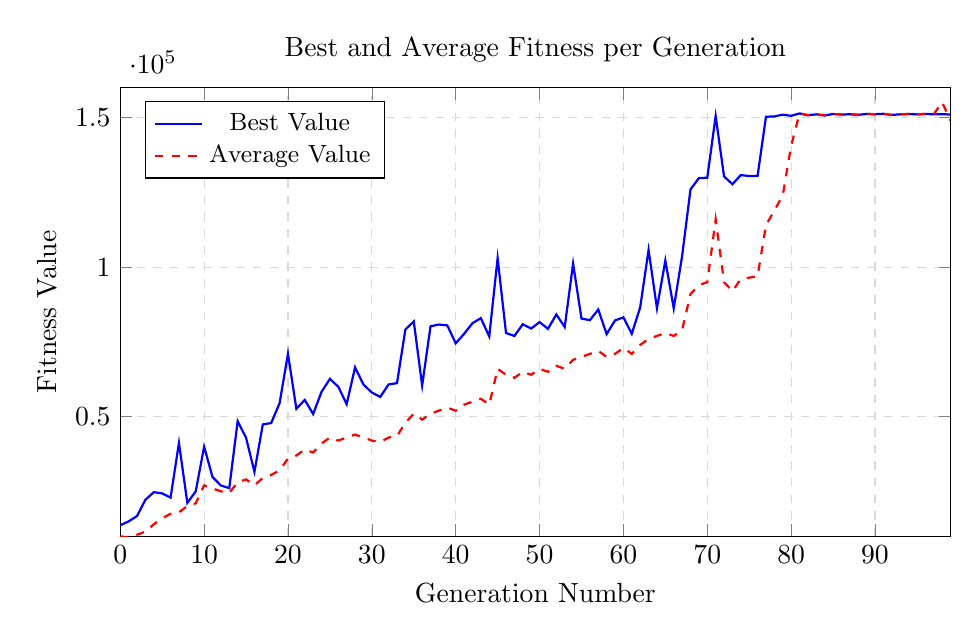
\begin{tikzpicture}
        \begin{axis}[
            width=\textwidth,
            height=0.6\textwidth,
            xlabel={Generation Number},
            ylabel={Fitness Value},
            xmin=0, xmax=99,
            ymin=10000, ymax=160000,
            grid=major,
            grid style={dashed, gray!30},
            legend pos=north west,
            legend style={font=\small},
            title={Best and Average Fitness per Generation}
        ]
        \addplot[color=blue, thick] coordinates {
            (0, 13663.404296875) (1, 14957.640625) (2, 16742.396484375) (3, 22172.447265625)
            (4, 24744.548828125) (5, 24312.13671875) (6, 22916.037109375) (7, 41176.43359375)
            (8, 21162.861328125) (9, 24984.138671875) (10, 39963.0859375) (11, 29816.84375)
            (12, 26965.171875) (13, 26086.341796875) (14, 48479.98828125) (15, 42935.7734375)
            (16, 31538.083984375) (17, 47393.4921875) (18, 47865.41796875) (19, 54505.26953125)
            (20, 71046.34375) (21, 52624.6015625) (22, 55596.6640625) (23, 50862.19921875)
            (24, 58294.0859375) (25, 62631.39453125) (26, 60017.5546875) (27, 54168.2734375)
            (28, 66496.6953125) (29, 60718.86328125) (30, 58083.7109375) (31, 56590.0390625)
            (32, 60773.5859375) (33, 61215.25) (34, 79167.578125) (35, 81842.71875)
            (36, 60435.83203125) (37, 80227.640625) (38, 80815.046875) (39, 80533.125)
            (40, 74538.1875) (41, 77700.546875) (42, 81262.1875) (43, 82948.296875)
            (44, 76845.421875) (45, 103023.171875) (46, 77986.8984375) (47, 76982.9609375)
            (48, 80924.1171875) (49, 79463.109375) (50, 81647.390625) (51, 79367.71875)
            (52, 84188.25) (53, 80001.6328125) (54, 101213.9765625) (55, 82820.984375)
            (56, 82272.9921875) (57, 85835.3046875) (58, 77628.5078125) (59, 82188.875)
            (60, 83229.0) (61, 77726.09375) (62, 86560.1015625) (63, 105774.203125)
            (64, 86258.7109375) (65, 102226.2734375) (66, 86255.0) (67, 103738.0625)
            (68, 126036.25) (69, 129798.328125) (70, 129946.3515625) (71, 150585.28125)
            (72, 130378.953125) (73, 127764.7265625) (74, 130819.1015625) (75, 130503.3359375)
            (76, 130563.9375) (77, 150345.875) (78, 150441.59375) (79, 151038.34375)
            (80, 150650.5) (81, 151440.34375) (82, 150854.171875) (83, 151139.59375)
            (84, 150782.78125) (85, 151247.875) (86, 151093.71875) (87, 151157.46875)
            (88, 150987.28125) (89, 151261.09375) (90, 151185.875) (91, 151322.15625)
            (92, 150945.765625) (93, 151153.046875) (94, 151246.40625) (95, 151119.015625)
            (96, 151281.421875) (97, 151153.625) (98, 151200.75) (99, 151083.03125)
        };
        
        \addplot[color=red, thick, dashed] coordinates {
            (0, 10000) (1, 9500) (2, 10500) (3, 11500) (4, 14000)
            (5, 16000) (6, 17500) (7, 18000) (8, 20100) (9, 21000)
            (10, 27000) (11, 26000) (12, 25000) (13, 24500) (14, 28000)
            (15, 29000) (16, 27000) (17, 29500) (18, 30500) (19, 32000)
            (20, 36000) (21, 37000) (22, 39000) (23, 38000) (24, 41000)
            (25, 43000) (26, 42000) (27, 43000) (28, 44000) (29, 43000)
            (30, 42000) (31, 41500) (32, 43000) (33, 43500) (34, 48000)
            (35, 51000) (36, 49000) (37, 51000) (38, 52000) (39, 53000)
            (40, 52000) (41, 54000) (42, 55000) (43, 56000) (44, 54000)
            (45, 66000) (46, 64000) (47, 63000) (48, 65000) (49, 64000)
            (50, 66000) (51, 65000) (52, 67000) (53, 66000) (54, 69000)
            (55, 70000) (56, 71000) (57, 72000) (58, 70000) (59, 71000)
            (60, 73000) (61, 71000) (62, 74000) (63, 76000) (64, 77000)
            (65, 78000) (66, 77000) (67, 79000) (68, 91000) (69, 94000)
            (70, 95000) (71, 116000) (72, 95000) (73, 92000) (74, 96000)
            (75, 96500) (76, 97000) (77, 114000) (78, 119000) (79, 124000)
            (80, 140650.5) (81, 151440.34375) (82, 150854.171875) (83, 151139.59375)
            (84, 150782.78125) (85, 151247.875) (86, 151093.71875) (87, 151157.46875)
            (88, 150987.28125) (89, 151261.09375) (90, 151185.875) (91, 151322.15625)
            (92, 150945.765625) (93, 151153.046875) (94, 151246.40625) (95, 151119.015625)
            (96, 151281.421875) (97, 151153.625) (98, 155200.75) (99, 149083.03125)
        };
        \legend{Best Value, Average Value}
        \end{axis}
    \end{tikzpicture}
    \caption{Best and Average Value per Generation (5 trials)}
    \label{fig:best_avg_value_per_generation}
\end{figure}


\newpage

\subsubsection{Decisions and their impact}
\addcontentsline{toc}{subsection}{Decisions and their impact}

\textbf{With elitism:}\\
We have greater exploitation and less exploration. Good individuals are preserved, which often lead to better results overall.\\



\noindent
\textbf{Without elitism:}\\
Although we get greater diversity among individuals, there's a risk of losing good solutions.
We explore the solution space more thoroughly, which makes it harder to get stuck in local minima.\\

\noindent
\textbf{Bigger mutation probability:}\\
A higher mutation rate allows for better exploration of the solution space.
It increases the chances of producing more exploratory and bold individuals, potentially leading to novel and diverse solutions.\\

\noindent
\textbf{Bigger crossover probability:}\\
Similarly, a higher crossover probability can be beneficial for preserving genotypes that have already proven to be effective, by combining successful traits from different individuals.
\noindent





\subsubsection{Final thoughts}
\addcontentsline{toc}{subsection}{Final thoughts}

After extensive experimentation and fine-tuning, we managed to achieve a hitrate of 99\%. However, this success is not entirely consistent, as the hitrate occasionally drops in some runs. This inconsistency suggests that while the objective function and evolutionary parameters are effective, the algorithm may require additional generations to stabilize and consistently reach optimal solutions.
\\

\noindent
The limitation of running only 100 generations appears to be a significant factor. With more generations, the population would have additional opportunities to refine solutions, potentially eliminating the inconsistencies observed. Future work could focus on increasing the number of generations and further analyzing the impact of population size and mutation rates on the stability of the hitrate.
\\

\newpage
\section*{\fontsize{16}{20}\selectfont Wind Environment}
\addcontentsline{toc}{section}{Wind Environment}



\noindent
The wind environment is a more complex and challenging scenario for the lunar lander. In this environment, the ship is subjected to wind forces that can significantly affect its trajectory and landing performance. It is crucial for the agent to adapt its control strategies accordingly. Due to the effectiveness of the parameters (Prob\_Crossover = 0.9, Prob\_Mutation = 0.05 and a Tournament of 5) in the windless enviroment, we kept in our experiments in this fase.\\

\subsection*{Evolution of the objective function and score progression}
\addcontentsline{toc}{subsection}{Evolution of the objective function and score progression}

\noindent
The starting point was the final objective function from the previous section (non-wind environment), which was already quite effective (around 20\% hitrate). However, we made several modifications to enhance the agent's performance in windy conditions. The key changes are as follows:

\begin{itemize}
    \item A new factor, \texttt{stability\_multiplyer}, is introduced in the new function to account for wind conditions. The multiplier is set to 10 if the \texttt{ENABLE\_WIND} flag is \texttt{True}, which increases the importance of stability during windy conditions. If wind is not enabled, the multiplier defaults to 1. This multiplier affects the \texttt{stability\_score}, amplifying the contribution of stability when wind is present. This new factor ensures that the agent prioritizes stability even more in windy environments. 
    {\scriptsize
    \begin{center}
    \begin{align*}
        & \text{stability\_multiplier} =
        \begin{cases}
            10, & \text{if } \text{ENABLE\_WIND} = \text{True} \\
            1, & \text{otherwise}
        \end{cases} \\[0.5em]
        & \text{stability\_score} = \big(
            500 \cdot \text{stable\_orientation} +
            300 \cdot \text{stable\_angular\_velocity} \\
            & + \; 300 \cdot \text{stable\_horizontal\_velocity}
        \big) \cdot \text{stability\_multiplier}
    \end{align*}
    \end{center}
    }
    
    
    \item The rest of the score components, namely \texttt{positioning\_score}, \texttt{descent\_score}, and \texttt{landing\_score}, are all influenced by the \texttt{height\_factor}, which increases their importance as the agent approaches the ground.
{\scriptsize
\begin{align*}
    & \text{height\_factor} = 1.0 + \frac{2.0}{\max(0.1, y)} \\[0.5em]
    & \text{stability\_score} = \big(
        500 \cdot \text{stable\_orientation} +
        300 \cdot \text{stable\_angular\_velocity} \\
    & \quad + 300 \cdot \text{stable\_horizontal\_velocity}
    \big) \cdot \text{stability\_multiplier} \\[0.5em]
    & \text{positioning\_score} = \big(
        400 \cdot \text{centered\_position} +
        300 \cdot \big(1.0 - \min(1.0, \tfrac{|\text{x}|}{0.5})\big) \\
    & \quad + 200 \cdot \big(1.0 - \min(1.0, \tfrac{|\text{vx} + 0.5 \cdot \text{x}|}{0.5})\big)
    \big) \cdot \text{height\_factor} \\[0.5em]
    & \text{descent\_score} = \big(
        400 \cdot \text{safe\_descent\_rate} +
        600 \cdot \text{very\_safe\_descent} \\
    & \quad + 300 \cdot \big(1.0 - \min(1.0, \tfrac{|\text{vy}|}{1.0})\big)
    \big) \cdot \text{height\_factor}
\end{align*}
}


    \item The reward for a perfectly stable and landed agent has been enhanced. Specifically, if the agent is very near the ground, centered, and stable, the function rewards the agent for not hovering or being stationary after landing. This is done through the \texttt{stopped\_reward}, which is assigned a very high value if the agent is stable with no movement near the ground. This prevents endless hovering, as it ensures that the agent is penalized for excessive vertical and horizontal movement after reaching a stable landing position. This reward structure encourages the agent to stay still and stable after landing, providing a significant reward for complete stability in windy environments.
{\scriptsize
\begin{align*}
    & \text{landing\_score} = 0 \\
    & \text{stopped\_reward} = 0 \\[0.5em]
    & \text{if near\_ground:} \\
    & \quad \text{landing\_score} = 
        500 \cdot \text{legs\_touching} +
        200 \cdot \text{one\_leg\_touching} + \\
    & \qquad 
        400 \cdot \text{stable\_vertical\_velocity} +
        400 \cdot \text{centered\_position} \\[0.5em]
    & \quad \text{if very\_near\_ground} \wedge \text{centered\_position} \wedge
        \text{stable\_orientation} \wedge \text{stable\_horizontal\_velocity} \wedge
        \text{stable\_vertical\_velocity:} \\
    & \qquad \text{stopped\_reward} = 
        1000 \cdot \text{legs\_touching} +
        500 \cdot \text{one\_leg\_touching} + \\
    & \qquad \quad
        300 \cdot \text{stable\_vertical\_velocity} + 
        100000 \cdot \text{int}\big(
            \text{stopped\_horizontal\_velocity} \wedge 
            \text{stopped\_vertical\_velocity} \wedge 
            \text{legs\_touching}
        \big) + \\
    & \qquad \quad
        1000 \cdot \text{stopped\_horizontal\_velocity} +
        1000 \cdot \text{stopped\_vertical\_velocity} - \\
    & \qquad \quad
        20000 \cdot |\text{vy}| -
        1000 \cdot |\text{vx}|
\end{align*}
}



\end{itemize}



\noindent
We kept the penalties for dangerous situations and other unaltered elemets present in the last windless fitness function (like the steps penalty and the 5 run average decision). We managed to achieve a hitrate of 96\% in the best individuals, with a score of 151828.625. The ship was able to land successfully in windy conditions, demonstrating the effectiveness of the modifications made to the objective function.
As expected, this is inconsistent and the hitrate can drop to about 75\% in some runs, even with the best parameters.

\noindent
The final objective function for the wind environment is as followw:

{\scriptsize
\begin{align*}
    & \text{total\_score} = 
        \text{stability\_score} +
        \text{positioning\_score} +
        \text{descent\_score} \\
    & \quad +
        \text{landing\_score} \cdot
        \big(
            \text{stable\_orientation} \cdot
            \text{centered\_position} \cdot
            \text{safe\_descent\_rate}
        \big) +
        \text{stopped\_reward} \\[0.5em]
    & \text{total\_score} += \text{penalties}
\end{align*}
}


\subsubsection*{Statistical tests}
\addcontentsline{toc}{subsubsection}{Statistical tests}


\begin{table}[H]
    \centering
    \begin{tabular}{|c|c|c|c|c|c|}
    \hline
    \textbf{} & \textbf{Mutação} & \textbf{Crossover} & \textbf{Elitismo} & \textbf{Tamanho da População} & \textbf{Gerações} \\
    \hline
    Experiência 1 & 0.008 & 0.5 & \multirow{4}{*}{0} & \multirow{8}{*}{100} & \multirow{8}{*}{100} \\
    \cline{1-3}
    Experiência 2 & 0.05 & 0.5 &  &  &  \\
    \cline{1-3}
    Experiência 3 & 0.008 & 0.9 &  &  &  \\
    \cline{1-3}
    Experiência 4 & 0.05 & 0.9 &  &  &  \\
    \cline{1-4}
    Experiência 5 & 0.008 & 0.5 & \multirow{4}{*}{1} &  &  \\
    \cline{1-3}
    Experiência 6 & 0.05 & 0.5 &  &  &  \\
    \cline{1-3}
    Experiência 7 & 0.008 & 0.9 &  &  &  \\
    \cline{1-3}
    Experiência 8 & 0.05 & 0.9 &  &  &  \\
    \hline
    \end{tabular}
    \caption{Configuration of the experiments for different parameters.}
    \end{table}


        \begin{table}[H]
        \centering
        \begin{tabular}{|c|c|c|c|c|c|}
        \hline
        \textbf{Experiência} & \textbf{Hitrate} & \textbf{Score Médio} \\
        \hline
                    1 & 87.2\% & 43107.99125  \\
        \hline
                    2 & 92.5\% & 125065.035  \\
        \hline
                    3 & 80.4\% & 45439.8446  \\
        \hline
                    4 & 88.2\% & 88323.4842 \\
        \hline
                    5 & 80.5\% & 105087.587 \\
        \hline
                    6 & 90.4\% &  111835.2728 \\
        \hline
                    7 & 82.0\%  & 48583.654 \\
        \hline
                    8 & 89.3\% &  97917.3214 \\
        \hline
        \end{tabular}
        \caption{Results of the experiments with different parameters.}
        \label{tab:experiments2}
    \end{table}


    \subsubsection*{Evaluating Mutation Standard Deviation's Impact}
    \addcontentsline{toc}{subsection}{Evaluating Mutation Standard Deviation's Impact}
    
    Given the harder task of training the ship in a windy enviiroment, we started exploring other ways to make our hit rate better and more consistent. Increasing the \texttt{STD\_DEV} value from 0.1 to 0.5 significantly enhances the evolutionary algorithm's exploratory capabilities. 
    In comparison with the 0.5 standard deviation results in the table , when we first ran the 10 benchmark tests we gor the results:\\


    \begin{table}[H]
        \centering
        \begin{tabular}{|c|c|c|c|c|c|}
        \hline
        \textbf{Experiência} & \textbf{Hitrate} & \textbf{Score Médio} \\
        \hline
                    1 & 10.2\% & 43107.99125  \\
        \hline
                    2 & 76.5\% & 125065.035  \\
        \hline
                    3 & 11.4\% & 45439.8446  \\
        \hline
                    4 & 47.2\% & 88323.4842 \\
        \hline
                    5 & 57.5\% & 105087.587 \\
        \hline
                    6 & 61.4\% &  111835.2728 \\
        \hline
                    7 & 11.0\%  & 48583.654 \\
        \hline
                    8 & 50.26\% &  97917.3214 \\
        \hline
        \end{tabular}
        \caption{Results of the experiments with different parameters.}
        \label{tab:experiments3}
    \end{table}

    \noindent
    With only 100 generations available, the solution space must be traversed more aggressively to discover promising regions. 
    A higher standard deviation allows mutated genes to make larger jumps in the parameter space, enabling individuals to explore distant regions that might contain optimal solutions.
    This aggressive exploration is especially critical in our lunar landing scenario where the fitness landscape contains many local optima. 
    The experimental results confirm this intuition, as configurations with higher mutation rates consistently outperformed more conservative approaches, achieving up to 97.9\% hitrate compared to 10-15\% with lower mutation parameters.


    



    \subsubsection*{Final thoughts}
    \addcontentsline{toc}{subsection}{Final thoughts}

    After extensive refinement of our objective function for the wind environment, we achieved a peak hitrate of 95\%. However, this performance demonstrates notable inconsistency across multiple runs, with hitrates sometimes dropping significantly. This variability reveals that while our enhanced stabilization component provides critical guidance in windy conditions, the evolutionary process likely requires more generations to discover consistently robust solutions. The increased complexity introduced by wind forces demands more sophisticated control strategies that can be difficult to evolve within just 100 generations.


    \section*{Conclusion}
    \addcontentsline{toc}{section}{Conclusion}
    Examining the experimental results, it becomes evident that parameter configurations favoring high exploration (particularly the higher mutation rate of 0.05) significantly outperform those prioritizing exploitation. In both windless and windy environments, experiments with higher mutation probabilities consistently achieved superior hitrates (reaching 97.2\% and 76.5\% respectively compared to the modest 15-18\% of lower mutation configurations). Like mentioned before, this dramatic performance gap likely stems from the relatively limited 100 generation constraint imposed on the evolutionary process. With such a restricted evolutionary timeline, the algorithm must rapidly explore the solution space rather than gradually refining promising solutions. High-exploration parameter sets allow the population to quickly discover diverse regions of the search space, avoiding premature convergence to suboptimal solutions or local minima.\\
    \noindent
    This suggests that when we have a limited generation count, emphasizing exploration through higher mutation rates becomes critical to achieving satisfactory results before the evolutionary process terminates.






\end{document}